% !TEX program = pdflatex

\documentclass{standalone}

\usepackage[utf8]{inputenc}
\usepackage[T1]{fontenc}
% \usepackage{fontspec}
% \usepackage{xunicode}
\usepackage{graphicx}
% \usepackage[a4paper,margin=20mm]{geometry}

% Polices
% \defaultfontfeatures{Mapping=tex-text}                              % Ligatures
% \setsansfont[BoldFont={Source Sans Pro Semibold}]{Source Sans Pro}  % Police sans-serif
% \usefonttheme[onlymath]{serif}                                      % Maths en serif




\begin{document}

\begin{minipage}{18cm}

\parbox[t]{.3\textwidth}{\centering%
  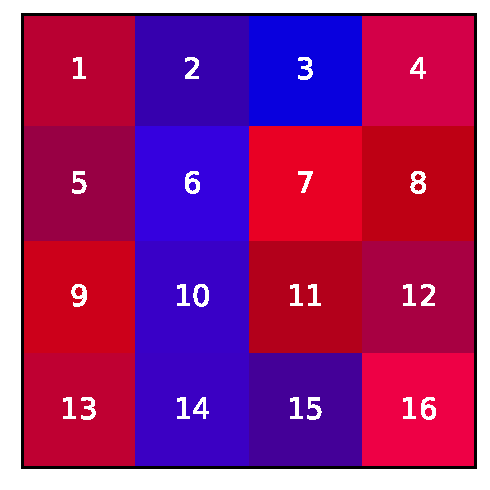
\includegraphics[scale=.55]{image.pdf}\\
  Image with bands red and blue.
  Numbers are the pixel indices.
}
\hfill
\parbox[t]{.3\textwidth}{\centering%
  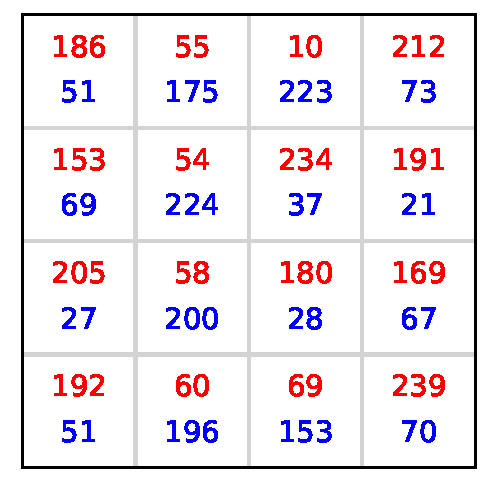
\includegraphics[scale=.55]{intensities.pdf}\\
  Intensities (red and blue) \\ of the pixels.
}
\hfill
\parbox[t]{.3\textwidth}{\centering%
  \raisebox{-5mm}{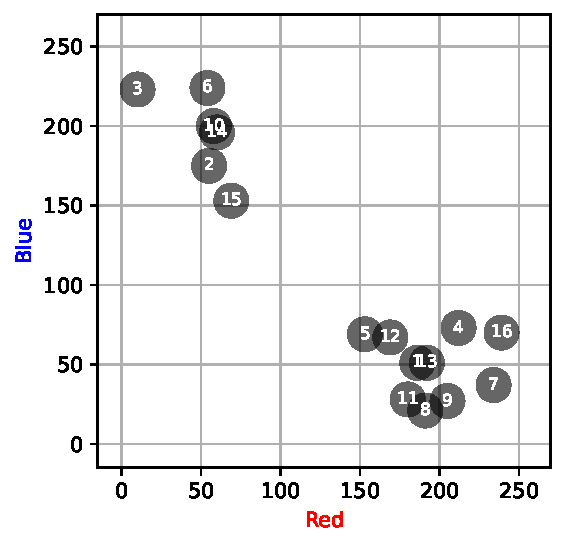
\includegraphics[scale=.55]{scatter.pdf}}\\
  Pixels plotted in \\ the (red,blue) space.
}

\bigskip
\begin{center}
  \parbox[t]{.18\textwidth}{\centering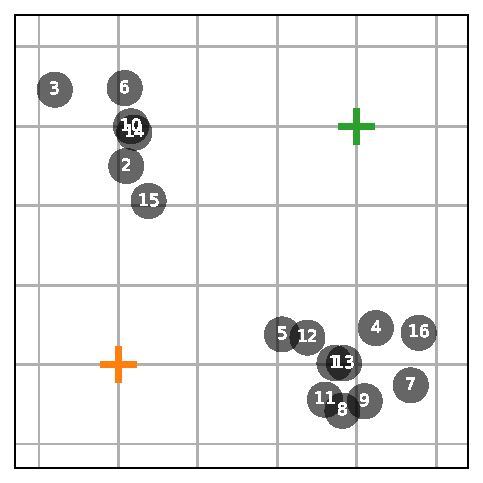
\includegraphics[width=.19\textwidth]{Initialisation.pdf}\\Initialization}\hfill
  \parbox[t]{.18\textwidth}{\centering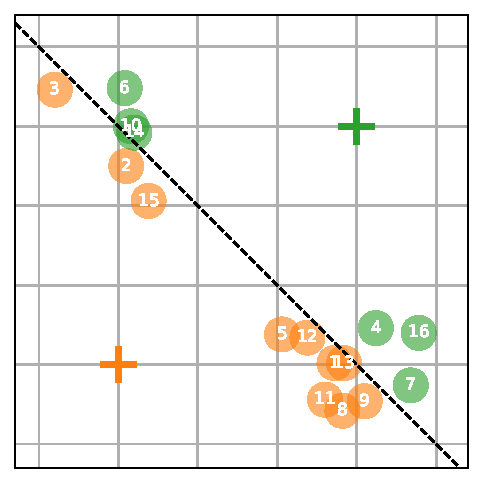
\includegraphics[width=.19\textwidth]{step-1A.pdf}\\Iteration 1\\Step A}\hfill
  \parbox[t]{.18\textwidth}{\centering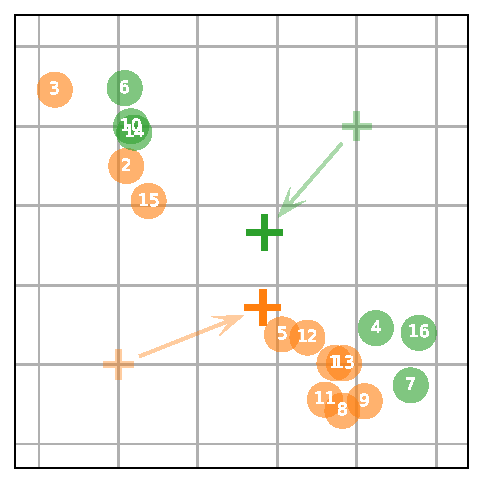
\includegraphics[width=.19\textwidth]{step-1B.pdf}\\Iteration 1\\Step B}\hfill
  \parbox[t]{.18\textwidth}{\centering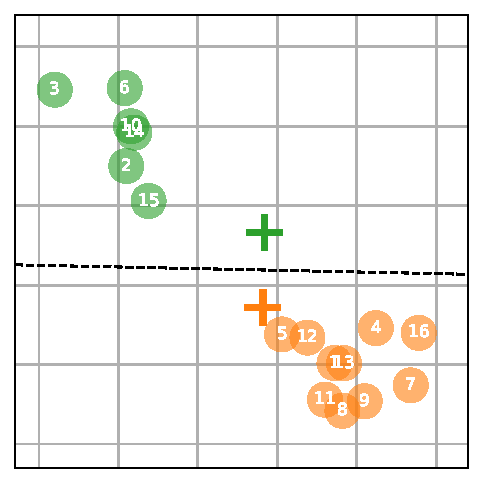
\includegraphics[width=.19\textwidth]{step-2A.pdf}\\Iteration 2\\Step A}\hfill
  \parbox[t]{.18\textwidth}{\centering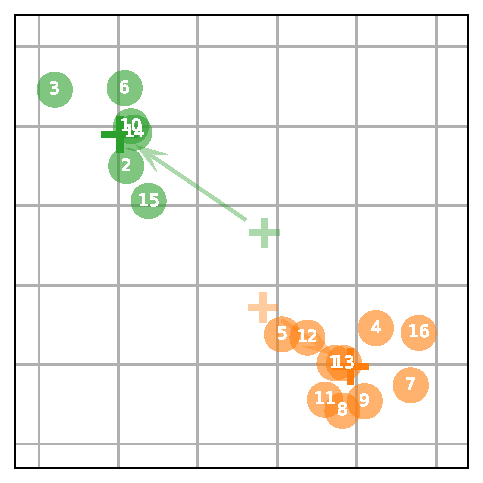
\includegraphics[width=.19\textwidth]{step-2B.pdf}\\Iteration 2\\Step B}\hfill
  \raisebox{15mm}{\Large$\cdots$}\\
  \bigskip
  Progression of the K-means algorithm
  (only the initialization and the first two iterations are illustrated).\\
  Centroids are represented by $+$,
  the dotted line indicates the boundary between the two classes.
\end{center}

\end{minipage}

\end{document}
